\documentclass{beamer}

\usetheme{Berlin}
%\usetheme{Ilmenau}
\usefonttheme{structurebold}

\title{The Mirai Botnet}
\author{Ulysses Butler, Thu Vo, and Tung Thai, Torey Clark}

\institute{ Truman State University \\ Binary Beasts }

\date{}

%https://www.usenix.org/system/files/conference/usenixsecurity17/sec17-antonakakis.pdf

%You are expected to read and analyze and dissect the information presented in the research paper, and if you look up online you might also be able to find PPT/Video presentation of the paper. Based on your understanding your team would prepare a research presentation that'd include the problem statement (issue), methodology (process), results including pros-cons of the research paper. You are expected to go above and beyond the assigned paper and present your "RESEARCHED" information in a concise manner about the topic.  Any sort of demo is highly encouraged but not required.

%The presentation would last 35 minutes so prepare accordingly and each team member is required to participate in presenting the material. You are also required to prepare a summary document in 800-1200 words, that presents the crux of the research problem and possible solutions. 

%Each team shall have 35 mins to present their research on their topic. You should include the problem statement, motivation, related works, background, contribution, evaluation, significance of the research paper along with your own research on the topic.

\begin{document}

\maketitle

\section{Introduction}

\begin{frame}
	\frametitle{The Paper}
	\begin{itemize}
		\item<+-> Title: \textit{Understanding the Mirai Botnet}
		\item<+-> \textit{The Proceedings of the 26th USENIX Security Symposium}
		\item<+-> This paper explores the Mirai botnet
		\item<+-> This botnet was responsible for one of the largest DDoS attacks every recorded.
		\item<+-> The purpose of this paper was to learn about how the botnet worked.
		\item<+-> Researchers from a number of institutions reversed engineered it to better understand how it spread
		\item<+-> This paper then proposes reforms that can be made to prevent this kind of attack in the future
	\end{itemize}
\end{frame}

\begin{frame}
	\frametitle{Contributions}
	\begin{itemize}
		\item<1-> Lead Author
		\begin{itemize}
			\item<1-> Zane Ma - University of Illinois Urbana-Champaign
		\end{itemize}
		\item<2-> This paper had help from many different authors
		\begin{itemize}
			\item<3-> Manos Antonakakis - Georgia Institute of Technology
			\item<3-> Tim April - Akamai Technologies
			\item<3-> Michael Bailey - University of Illinois Urbana-Champaign
			\item<3-> Matthew Bernhard - University of Michigan
			\item<3-> Elie Bursztein - Google
			\item<3-> Jaime Cochran - Cloudflare
			\item<3-> Zakir Durumeric - University of Michigan
			\item<3-> J. Alex Halderman - University of Michigan
		\end{itemize}
	\end{itemize}
\end{frame}

\begin{frame}
	\frametitle{Contributions Cont.}
	\begin{itemize}
		\item<1-> Continued...
		\begin{itemize}
			\item<1-> Luca Invernizzi - Google
			\item<1-> Michalis Kallitsis - Merit Network
			\item<1-> Deepak Kumar - University of Illinois Urbana-Champaign
			\item<1-> Chaz Lever - Georgia Institute of Technology
			\item<1-> Joshua Mason - University of Illinois Urbana-Champaign
			\item<1-> Damian Menscher - Google
			\item<1-> Chad Seaman - Akamai Technologies
			\item<1-> Nick Sullivan - Cloudflare
			\item<1-> Kurt Thomas - Google
			\item<1-> Yi Zhou - University of Illinois Urbana-Champaign
		\end{itemize}
	\end{itemize}
\end{frame}

\section{Spreading}

\begin{frame}
	\frametitle{Bootstraping}
	\begin{itemize}
		\item<+-> August 1, 2016: Servers owned by DataWagon began a preliminary scan.
		\begin{itemize}
			\item<+-> DataWagon is a bulletproof web hosting provider.
			\item<+-> Users are allowed to upload and distribute almost anything using their service.
		\end{itemize}
		\item<+-> After this scan, the botnet started infecting computers
		\begin{itemize}
			\item<+-> 1 minute -  800 infected devices
			\item<+-> 10 minutes - 11,000 infected devices
			\item<+-> 20 hours - 65,000 infected devices
			\item<+-> Held steady at around 100,000 to 200,000 infections
			\item<+-> In December 2016, it peaked at 600,000 devices before beginning to fade
		\end{itemize}
	\end{itemize}
\end{frame}

\begin{frame}
	\frametitle{Spreading}
	\begin{columns}
		\column{0.5\linewidth}
			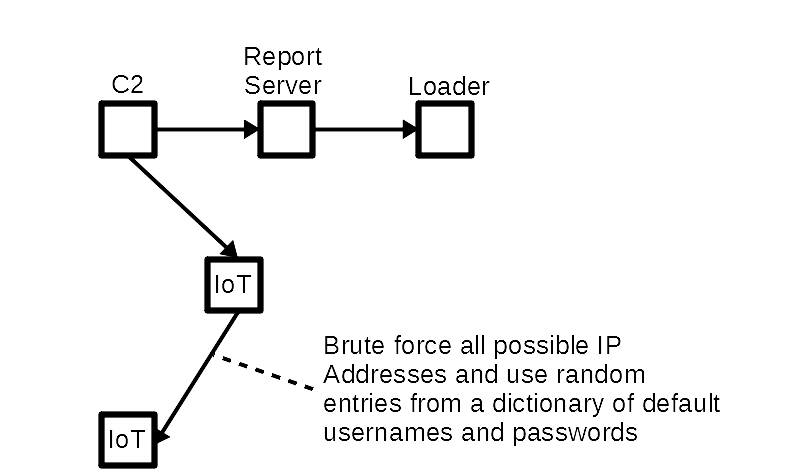
\includegraphics[width=\textwidth]{fig1.png}
		\column{0.5\linewidth}
			\begin{itemize}
				\item<+-> A member of the botnet begins scanning scanning ports on all IPv4 addresses
				\item<+-> It scans to find open ports for SSH, Telnet, FTP, and other protocols
				\item<+-> It would then use a dictionary attack to brute force into the machine
				\item<+-> These were small dictionaries, containing 60 to about 200 credentials
			\end{itemize}
	\end{columns}
\end{frame}

\begin{frame}
	\frametitle{Spreading}
	\begin{columns}
		\column{0.5\linewidth}
			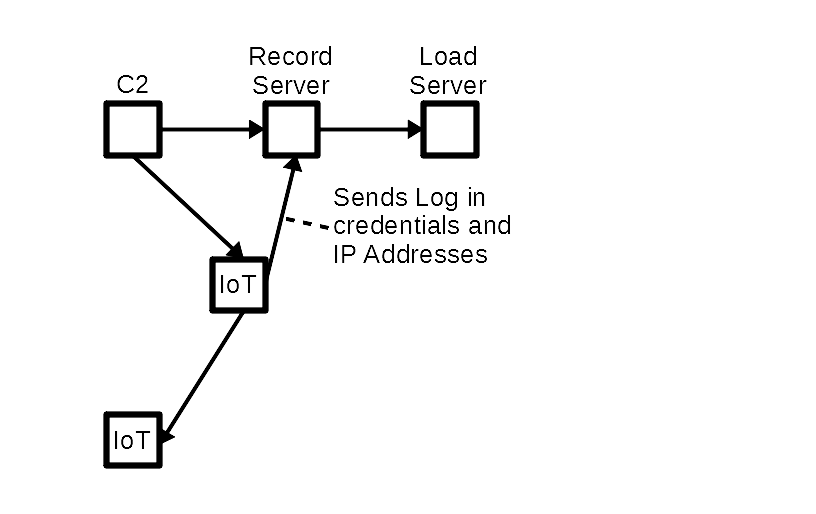
\includegraphics[width=\textwidth]{fig2.png}
		\column{0.5\linewidth}
			\begin{itemize}
				\item<+-> The address and credentials of the victim machines where then sent to a report server
				\item<+-> This information could later be used by the Command and Control (C2) server
			\end{itemize}
	\end{columns}
\end{frame}

\begin{frame}
	\frametitle{Spreading}
	\begin{columns}
		\column{0.5\linewidth}
			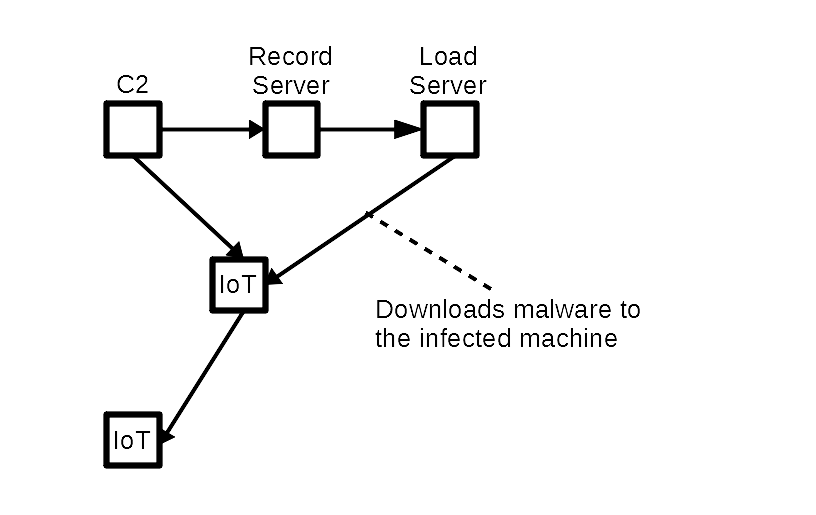
\includegraphics[width=\textwidth]{fig3.png}
		\column{0.5\linewidth}
			\begin{itemize}
				\item<+-> The records server then sent this information to the load program
				\item<+-> This program would download a binary onto the victim and run the program
			\end{itemize}
	\end{columns}
\end{frame}

\begin{frame}
	\frametitle{Loading the Binary}
	\begin{itemize}
		\item<+-> The aforementioned loader program downloaded an architecture specific binary
		\item<+-> The machine would then run the binary and change the process information to make it harder to detect
		\item<+-> The binary is then deleted.
		\begin{itemize}
			\item<+-> This means infections won't carry across reboots
		\end{itemize}
		\item<+-> Once the victim is infected, it starts scanning
		\begin{itemize}
			\item<+-> It would specifically avoid scanning servers owned by major corporations or the government
			\item<+-> These entities would likely be too secure for this simple attack
			\item<+-> This also allowed the bot to keep a lower profile
			\item<+-> These organizations would be much more likely to start search for and exploiting weaknesses in the malware if it infected their machines
		\end{itemize}
	\end{itemize}
\end{frame}

\section{Exploiting IoT}

\begin{frame}[fragile]
	\frametitle{Internet of Things Security}
	\begin{itemize}
		\item<+-> The Internet of Things
		\begin{itemize}
			\item<+-> Includes security cameras, routers, network-access storage, TV receivers, etc.
			\item<+-> Typically embedded systems that aren't powerful
		\end{itemize}
		\item<+-> Manufactures neglect security
		\begin{itemize}
			\item<+-> Many manufactures use one user name and password
			\item<+-> Common passwords are frequent. \verb|password|, \verb|admin|, etc.
			\item<+-> Some devices even have credentials hard coded in firmware
			\item<+-> Most companies don't have the infrastructure to release patches for these systems
		\end{itemize}
		\item<+-> This allowed the bot to easily infect a large number of machines
	\end{itemize}
\end{frame}

\begin{frame}
	\frametitle{Disadvantages}
	\begin{itemize}
		\item<+-> These less powerful devices also hurt Mirai's growth
		\begin{itemize}
			\item<+-> Mirai had a doubling time of 75-minutes
			\begin{itemize}
				\item<+-> Compare to 37-minutes for Code-Red
				\item<+-> 9-minutes for Blaster
			\end{itemize}
			\item<+-> Most bots scanned at less than 250 bytes per second
			\item<+-> Much slower than other bot nets
			\item<+-> SQL Slammer was about 6000 times faster at 1.5 megabytes per second
		\end{itemize}
		\item<+-> Most devices were found in low bandwidth countries
		\begin{itemize}
			\item<+-> Most infected devices were from South America and South-east Asia
			\item<+-> Brazil, Colombia, and Vietnam hosted most of the bots
		\end{itemize}
	\end{itemize}
\end{frame}

\section{Attacking}

\begin{frame}
    \frametitle{How DDoS Works}
    \begin{itemize}
        \item How to DDoS for Dummies
            \begin{itemize}
                \item<+-> A DDoS seeks to restrict a servers capabilities to respond to users by flooding it with requests from multiple different machines.
                \item<+-> DDoS attacks are more difficult to protect against compared to a DOS attack because it is difficult to blacklist multiple IP Addresses and distinguish between real requests and the attack.
            \end{itemize}
    \end{itemize}
\end{frame}

\begin{frame}
    \frametitle{Volumetric Attacks}
        \begin{itemize}
            \item Volumetric Attacks consist of a flooding a server with request packets to overwhelm its ability to respond. Volumetric attacks require little work to generate a high count of requests. With requests from multiple machines, it is difficult to prevent or dampen an attack on a server.
    \end{itemize}
\end{frame}
\begin{frame}
    \frametitle{Protocal Attacks}
     \begin{itemize}
            \item <+->Protocol Attacks seek to disable a server by exloiting a weakness in a protocl. SYN flood attacks TCP by exploiting the three-way handshake process to create a backlogged queue. Ping attacks uses a large number of pings to attack a server. UDP floods send massive amounts of packets to random ports to overwhelm the queue of responses.
        \end{itemize}
\end{frame}

\begin{frame}
    \frametitle{Application Layer Attacks}
        \begin{itemize}
            \item<+-> Application layer attacks attempt to exploit the layer of human interaction with a machine. These attacks are nearly indistinguishable from real user interaction. They requires far less resources to execute this attack than it takes to prevent that attack. This makes these attacks resource efficient for an attacker.
    \end{itemize}
\end{frame}
\begin{frame}
    \frametitle{}
    \begin{itemize}
        \item<+-> Most attacks were orchestrated against targets in the United States(50.3\%), France(6.6\%), and the UK(6.1\%).
        \item<+-> Mirai could also target particular ports to affect specific services. Of the attacks on specified ports, the most common ones attacked were 80(HTTP, 37.5\%), 25565(Minecraft, 9.2\%), 443(HTTPS, 6.4\%), and 23594(Runescape, 3.4\%).
        \item<+-> Several Mirai C2 servers were attacked by some of its other C2 servers. These are from renting DDoS attackers against other renting DDoS attackers.
    \end{itemize}
\end{frame}

\begin{frame}
    \frametitle{Attacks}
	\begin{itemize}
		\item<+->General Targets by Mirai
			\begin{itemize}
				\item<+-> Multiple DDoS attacks against a variety of targets
				\item<+-> Game Servers (primarily Minecraft and Runescape)
				\item<+-> Political Websites, anti-DDoS protectors
			\end{itemize}
		\item<+-> Notable Targets
			\begin{itemize}
				\item<+-> Krebs on Security - largest reported DDos attack to that point
				\item<+-> Dyn - DNS attack disrupted access for Amazon, Github, Netflix, Twitter, and others
				\item<+-> Lonestar Cell - most attacked target, destroyed internet capabilities in Liberia
			\end{itemize}
	\end{itemize}
\end{frame}

\section{Open Source}

\begin{frame}
	\frametitle{Releasing the Source Code}
	\begin{itemize}
		\item<+-> The source code was released on September 30, 2016
		\item<+-> A user named ``Anna-senpai'' released the source code for free on hackerforums.net
		\item<+-> This spawned a number of copycat attacks with variations on the original bot
		\begin{itemize}
			\item<+-> Many included new exploits, modified dictionaries, and different IP blacklists
		\end{itemize}
		\item<+-> These botnets eventually starting competing
		\begin{itemize}
			\item<+-> Killing processes started by similar bots
			\item<+-> Closing the ports used to attack the machine
			\item<+-> At various points, competing command and control servers were subject to DDoS attacks
		\end{itemize}
	\end{itemize}
\end{frame}

\section{Defending}
\begin{frame}
    \frametitle{Defense Against the Dark Arts}
    \begin{itemize}
        \item<+-> Industry Improvements
            \begin{itemize}
                \item<+-> Randomized default passwords 
                \item<+-> Closed ports on default
                \item<+-> Employ Automatic Updates and Self-Monitoring
                \item<+-> Creating Standard for Model and Firmware identification
            \end{itemize}
        \item<+-> User Improvements
            \begin{itemize}
                \item<+-> Create good secure credentials and not use the defaults
                \item<+-> Purchase from reputable and secure companies
                \item<+-> Replace old and unsupported devices
            \end{itemize}
    \end{itemize}
\end{frame}

\begin{frame}
    \frametitle{Defense Against the Dark Arts}
    \begin{itemize}
        \item Randomized default passwords prevent attackers from employing a dictionary of default passwords.
        \item Having ports not used default to closed mitigates the chances of a successful attack.
        \item Automatic updates prevent users from refusing updates during hours of use and keeps systems secure against previous exploits. Bug bounties encourage the community to find and report all possible exploits to be patched.
        \item Standards for model and version identification allow server admins to easily see any and all machines that have known vulnerabilities.
    \end{itemize}
\end{frame}
\begin{frame}
    \frametitle{Defense Against the Dark Arts}
    \begin{itemize}
        \item Users should create secure usernames and passwords for all devices to mitigate the chance of it being hacked using brute force.
        \item Smart purchases from known and trusted companies that prioritize security of their manufactured devices acts as a deterrent from would be attackers.
        \item Old and unsupported devices should be replaced with newer models that conform with current security standards and have strong customer support.
    \end{itemize}
    
\end{frame}

\section{Further Research}

\begin{frame}
	\frametitle{Origin of Mirai}
	\begin{itemize}
		\item<+-> Mirai was created by 3 computer science students
	\end{itemize}
\end{frame}

\section{Conclusion}

\begin{frame}
	\frametitle{Conclusion}
	\begin{itemize}
		\item<+-> Mirai was a centralized botnet that was responsible for some of the largest DoS attacks every recorded.
		\item<+-> This bot was relatively simple with small dictionaries
		\item<+-> They creators of this bot exploited the security negligence of hardware manufactures
		\item<+-> They were able to quickly take over a large number of IoT devices
		\item<+-> This attack served as a wake up call, prompting reform in these industries
	\end{itemize}
\end{frame}

\end{document}
